% gps_estimation_deep.tex — Deep-dive on GPS target estimation
% Appendix K
% ─────────────────────────────────────────────────────────────────────

\section{GPS Target Estimation: A Deep Dive}\label{sec:gps-deep}

Translating a bounding-box centre in a camera frame into a world-referenced GPS coordinate is arguably the most error-sensitive computation in the entire SAR pipeline.  Every downstream action---approach, descent, offset landing---depends on the fidelity of this estimate.  A single observation combines at least six independent noise sources (GPS receiver, barometer, compass, camera intrinsics, camera extrinsics, and timing lag), and the engineering challenge is to fuse many such observations into a position estimate precise enough to guide a safe offset landing.  This appendix presents the full mathematical derivation of the pixel-to-GPS projection, catalogues and quantifies the dominant error sources, compares three estimation strategies and four fusion algorithms, describes the spatial clustering algorithm that handles multi-target scenarios, and reports the empirical accuracy obtained from both DJI flight-video replay and interactive simulator trials.

% =====================================================================
\subsection{Strategy Roadmap}\label{sec:strategy-roadmap}

Before diving into the mathematics, it is useful to preview the overall estimation strategy and how accuracy improves through the mission.  The system faces a fundamental challenge: the camera sees pixels, but the mission needs GPS coordinates.  A single GPS reading has \SIrange{2}{3}{\metre} uncertainty, and the pixel-to-GPS projection amplifies this through multiple error sources (roll/pitch, timing lag, calibration).  Three estimation strategies were evaluated (Section~\ref{sec:three-strategies}), and the mission architecture was designed so that accuracy improves progressively through the state machine:

\begin{table}[ht]
  \centering
  \caption{Target position accuracy progression through mission states.  CEP$_{50}$ is the radius containing 50\% of estimates.  $N$ is the number of fused observations at each stage.}
  \label{tab:accuracy-progression}
  \begin{tabular}{llccl}
    \toprule
    \textbf{State} & \textbf{Drone Condition} & \textbf{CEP$_{50}$} & \textbf{$N_\mathrm{obs}$} & \textbf{Dominant Error} \\
    \midrule
    SEARCH     & Moving, $10^{\circ}$ pitch, 35\,m & $\sim$\SI{7}{\metre} & 1--5     & Roll/pitch projection \\
    CENTERING  & Decelerating $\to$ hover, 35\,m   & $\sim$\SI{3}{\metre} & 5--20    & GPS receiver noise \\
    VERIFY     & Stationary hover, 15\,m           & $\sim$\SI{1.5}{\metre} & 20--48 & GPS averaging limit \\
    \bottomrule
  \end{tabular}
\end{table}

\noindent The key insight is that the mission procedure itself---centering the target in the frame and hovering---eliminates the largest error sources \emph{without any software correction}.  When the target is at the optical centre, pixel offset is zero, and every multiplicative error in the projection chain (GSD, focal length, yaw, lens distortion) is multiplied by zero and vanishes (Section~\ref{sec:two-approaches}).  The only remaining error is the drone's own GPS accuracy, which is reduced by $\sqrt{N}$ through multi-frame averaging.

% =====================================================================
\subsection{Problem Statement}\label{sec:gps-problem}

The detection subsystem (Section~\ref{sec:cv}) produces, for each frame, a bounding-box centre $(u,v)$ in pixel coordinates together with a confidence score.  Mapping this to a WGS\,84 latitude--longitude pair requires five additional quantities, each of which carries measurement uncertainty:

\begin{enumerate}
  \item The drone's own GPS position $(\phi_d, \lambda_d)$, subject to receiver noise and latency.
  \item The barometric altitude $h$ above ground level, subject to drift and calibration error.
  \item The magnetometer heading $\psi$, subject to hard-/soft-iron distortion and motor interference.
  \item The camera intrinsics---focal length $f$, sensor width $w_s$, and image dimensions $W \times H$---subject to calibration residuals and lens distortion.
  \item The camera extrinsics---its mounting angle relative to nadir---subject to mechanical tolerance.
\end{enumerate}

\noindent A single observation therefore combines at least six independent noise sources.  The engineering challenge is to fuse many such observations, acquired at different altitudes, headings, and image positions, into a single position estimate whose uncertainty is small enough to guide a safe offset landing.

% =====================================================================
\subsection{Detection-to-GPS Pipeline Overview}\label{sec:pipeline-overview}

\usetikzlibrary{shapes.geometric, arrows.meta, positioning, calc, fit}

The complete detection-to-GPS pipeline traverses 15~stages, grouped into four functional categories: image preprocessing (blue), neural network inference (green), coordinate transformation (orange), and validation/state management (red).  Figure~\ref{fig:pipeline-flow} shows the full data flow from raw sensor capture to a validated GPS estimate, annotated with data shapes, timing, and error contributions at each stage.

\begin{figure}[H]
  \centering
  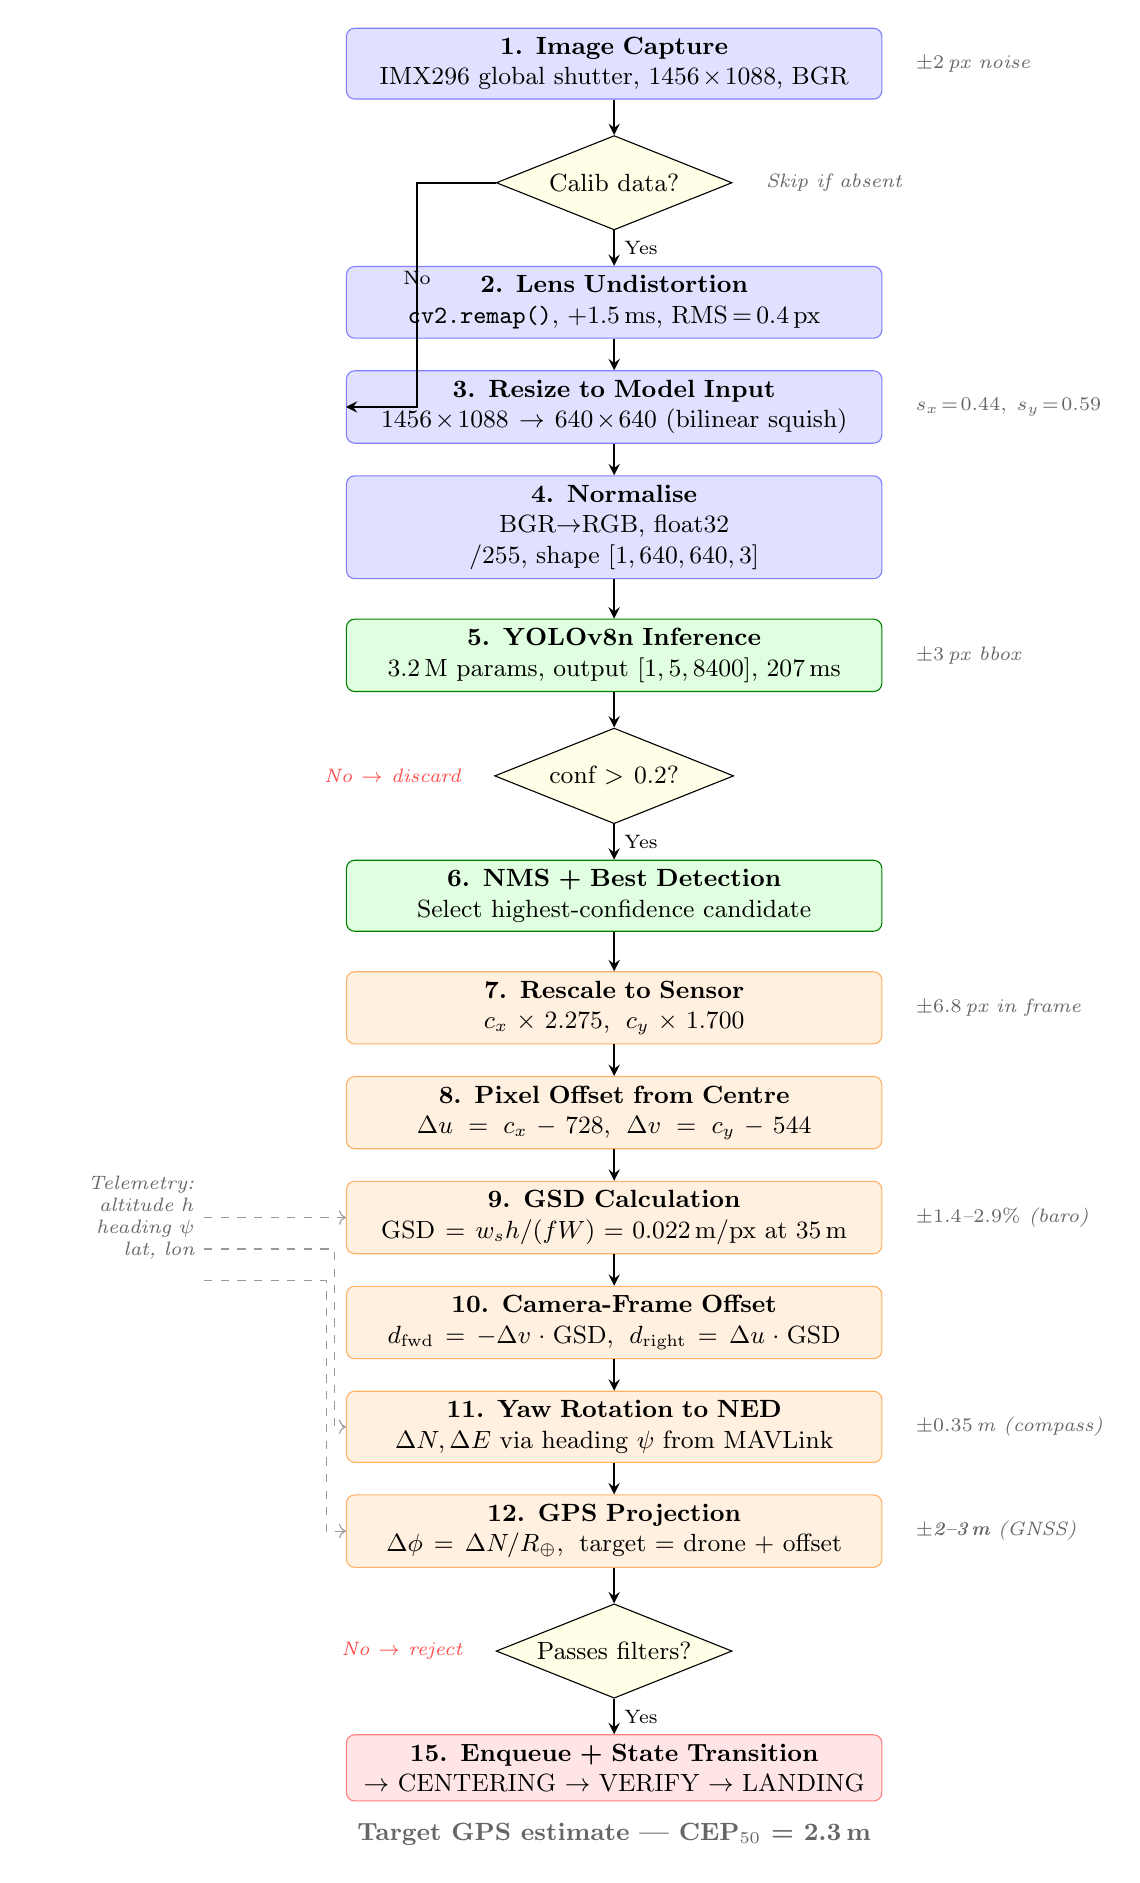
\begin{tikzpicture}[
    process/.style={rectangle, rounded corners=3pt, minimum width=6.8cm, minimum height=0.7cm, text centered, draw=black, font=\small, text width=6.5cm},
    imgproc/.style={process, fill=blue!12, draw=blue!50},
    inference/.style={process, fill=green!12, draw=green!50!black},
    coordtx/.style={process, fill=orange!12, draw=orange!60},
    validate/.style={process, fill=red!10, draw=red!50},
    decision/.style={diamond, aspect=2.5, draw=black, fill=yellow!10, font=\small, inner sep=1pt, text width=2.2cm, text centered},
    annot/.style={font=\scriptsize\itshape, text=black!60},
    arr/.style={thick, ->, >=stealth},
    node distance=0.52cm
  ]
    % --- Image Preprocessing (Blue) ---
    \node[imgproc] (s1) {\textbf{1. Image Capture}\\ IMX296 global shutter, $1456\!\times\!1088$, BGR};
    \node[annot, right=0.3cm of s1.east, anchor=west] {$\pm2$\,px noise};

    \node[decision, below=0.45cm of s1] (d2) {Calib data?};
    \node[imgproc, below=0.45cm of d2] (s2) {\textbf{2. Lens Undistortion}\\ \texttt{cv2.remap()}, +1.5\,ms, RMS\,=\,0.4\,px};
    \node[annot, right=0.3cm of d2.east, anchor=west] {Skip if absent};

    \node[imgproc, below=0.4cm of s2] (s3) {\textbf{3. Resize to Model Input}\\ $1456\!\times\!1088 \to 640\!\times\!640$ (bilinear squish)};
    \node[annot, right=0.3cm of s3.east, anchor=west] {$s_x\!=\!0.44,\; s_y\!=\!0.59$};

    \node[imgproc, below=0.4cm of s3] (s4) {\textbf{4. Normalise}\\ BGR$\to$RGB, float32 $/255$, shape $[1,640,640,3]$};

    % --- Inference (Green) ---
    \node[inference, below=0.5cm of s4] (s5) {\textbf{5. YOLOv8n Inference}\\ 3.2\,M params, output $[1,5,8400]$, 207\,ms};
    \node[annot, right=0.3cm of s5.east, anchor=west] {$\pm3$\,px bbox};

    \node[decision, below=0.45cm of s5] (d6) {conf $> 0.2$?};
    \node[inference, below=0.45cm of d6] (s6) {\textbf{6. NMS + Best Detection}\\ Select highest-confidence candidate};
    \node[annot, left=0.3cm of d6.west, anchor=east] {\color{red!70}No $\to$ discard};

    % --- Coordinate Transform (Orange) ---
    \node[coordtx, below=0.5cm of s6] (s7) {\textbf{7. Rescale to Sensor}\\ $c_x \!\times\! 2.275$,\; $c_y \!\times\! 1.700$};
    \node[annot, right=0.3cm of s7.east, anchor=west] {$\pm6.8$\,px in frame};

    \node[coordtx, below=0.4cm of s7] (s8) {\textbf{8. Pixel Offset from Centre}\\ $\Delta u = c_x - 728$,\; $\Delta v = c_y - 544$};

    \node[coordtx, below=0.4cm of s8] (s9) {\textbf{9. GSD Calculation}\\ $\mathrm{GSD} = w_s h / (f W)$ = 0.022\,m/px at 35\,m};
    \node[annot, right=0.3cm of s9.east, anchor=west] {$\pm1.4$--$2.9\%$ (baro)};

    \node[coordtx, below=0.4cm of s9] (s10) {\textbf{10. Camera-Frame Offset}\\ $d_\mathrm{fwd} = -\Delta v \cdot \mathrm{GSD}$,\; $d_\mathrm{right} = \Delta u \cdot \mathrm{GSD}$};

    \node[coordtx, below=0.4cm of s10] (s11) {\textbf{11. Yaw Rotation to NED}\\ $\Delta N,\Delta E$ via heading $\psi$ from MAVLink};
    \node[annot, right=0.3cm of s11.east, anchor=west] {$\pm0.35$\,m (compass)};

    \node[coordtx, below=0.4cm of s11] (s12) {\textbf{12. GPS Projection}\\ $\Delta\phi = \Delta N / R_\oplus$,\; target = drone + offset};
    \node[annot, right=0.3cm of s12.east, anchor=west] {\textbf{$\pm$2--3\,m} (GNSS)};

    % --- Validation (Red) ---
    \node[decision, below=0.45cm of s12] (d14) {Passes filters?};
    \node[validate, below=0.45cm of d14] (s15) {\textbf{15. Enqueue + State Transition}\\ $\to$ CENTERING $\to$ VERIFY $\to$ LANDING};
    \node[annot, left=0.3cm of d14.west, anchor=east] {\color{red!70}No $\to$ reject};

    % --- Arrows ---
    \draw[arr] (s1) -- (d2);
    \draw[arr] (d2) -- (s2) node[midway, right, font=\scriptsize] {Yes};
    \draw[arr] (d2.west) -- +(-1.0,0) |- (s3.west) node[near start, above, font=\scriptsize] {No};
    \draw[arr] (s2) -- (s3);
    \draw[arr] (s3) -- (s4);
    \draw[arr] (s4) -- (s5);
    \draw[arr] (s5) -- (d6);
    \draw[arr] (d6) -- (s6) node[midway, right, font=\scriptsize] {Yes};
    \draw[arr] (s6) -- (s7);
    \draw[arr] (s7) -- (s8);
    \draw[arr] (s8) -- (s9);
    \draw[arr] (s9) -- (s10);
    \draw[arr] (s10) -- (s11);
    \draw[arr] (s11) -- (s12);
    \draw[arr] (s12) -- (d14);
    \draw[arr] (d14) -- (s15) node[midway, right, font=\scriptsize] {Yes};

    % --- Side inputs ---
    \node[annot, left=1.8cm of s9.west, anchor=east, text width=2cm, align=right] (telem) {Telemetry:\\altitude $h$\\heading $\psi$\\lat, lon};
    \draw[->, dashed, thin, black!40] (telem.east) -- (s9.west);
    \draw[->, dashed, thin, black!40] (telem.east) ++(0,-0.4) -| ($(s11.west)+(-0.15,0)$) -- (s11.west);
    \draw[->, dashed, thin, black!40] (telem.east) ++(0,-0.8) -| ($(s12.west)+(-0.25,0)$) -- (s12.west);

    % --- Output annotation ---
    \node[annot, below=0.15cm of s15, font=\small\bfseries] {Target GPS estimate --- CEP$_{50}$ = 2.3\,m};

  \end{tikzpicture}
  \caption{Complete 15-stage detection-to-GPS pipeline.  Blue: image preprocessing; green: neural network inference; orange: coordinate transformation; red: validation and state management.  Grey annotations show error contributions; dashed lines show telemetry inputs.  The confidence decision diamond and validation filter diamond are the two branch points where data may be discarded.}
  \label{fig:pipeline-flow}
\end{figure}

% =====================================================================
\subsection{Pixel-to-GPS Mathematics}\label{sec:gps-math}

\subsubsection{Ground Sampling Distance}

Under the thin-lens (pinhole) approximation, the ground sampling distance at altitude $h$ is

\begin{equation}\label{eq:gsd-deep}
  \mathrm{GSD}(h) = \frac{w_s \cdot h}{f \cdot W}
  \qquad [\text{m\,px}^{-1}]
\end{equation}

\noindent where $w_s = \SI{5.02}{\milli\metre}$ (IMX296 sensor width), $f = \SI{5.46}{\milli\metre}$ (calibrated focal length), and $W = 1456$\,px (native image width).  Table~\ref{tab:gsd-altitude} lists the resulting GSD and ground footprint at the three operational altitudes.

\begin{table}[ht]
  \centering
  \caption{Ground sampling distance and footprint at key mission altitudes.}
  \label{tab:gsd-altitude}
  \begin{tabular}{rcccc}
    \toprule
    \textbf{Altitude} & \textbf{GSD} & \textbf{Footprint} & \textbf{Dummy size} & \textbf{Dummy (px)} \\
    (m) & (mm\,px$^{-1}$) & (m $\times$ m) & (m) & (approx.) \\
    \midrule
    10  & 6.3  & $9.2 \times 6.9$   & 1.8 & 286 \\
    15  & 9.5  & $13.8 \times 10.3$ & 1.8 & 190 \\
    35  & 22.1 & $32.2 \times 24.0$ & 1.8 & 81  \\
    50  & 31.6 & $46.0 \times 34.3$ & 1.8 & 57  \\
    \bottomrule
  \end{tabular}
\end{table}

\subsubsection{Body-Frame Projection}

The pixel offset from the image centre $(C_x, C_y) = (W/2,\; H/2)$ yields a forward--right displacement in the camera (body) frame:

\begin{equation}\label{eq:body-deep}
  d_\mathrm{fwd} = -(v - C_y)\,\mathrm{GSD},
  \qquad
  d_\mathrm{right} = (u - C_x)\,\mathrm{GSD}
\end{equation}

\noindent The negative sign on the forward axis accounts for the image convention where $v$ increases downward (southward in a north-facing camera).

\subsubsection{Heading Rotation}

The body-frame offset is rotated into the geographic North--East frame using the drone's heading angle $\psi$ (measured clockwise from North):

\begin{equation}\label{eq:rotation-deep}
  \begin{pmatrix} \Delta N \\ \Delta E \end{pmatrix}
  =
  \begin{pmatrix} \cos\psi & -\sin\psi \\ \sin\psi & \phantom{-}\cos\psi \end{pmatrix}
  \begin{pmatrix} d_\mathrm{fwd} \\ d_\mathrm{right} \end{pmatrix}
\end{equation}

\subsubsection{WGS\,84 Conversion}

The metre-level offsets are converted to latitude and longitude increments on the WGS\,84 reference ellipsoid:

\begin{equation}\label{eq:wgs84-deep}
  \Delta\phi = \frac{\Delta N}{R_\oplus} \cdot \frac{180}{\pi},
  \qquad
  \Delta\lambda = \frac{\Delta E}{R_\oplus \cos\phi_d} \cdot \frac{180}{\pi}
\end{equation}

\noindent where $R_\oplus = \SI{6378137}{\metre}$ is the WGS\,84 semi-major axis and $\phi_d$ is the drone's current latitude.  The estimated target position is $(\phi_d + \Delta\phi,\; \lambda_d + \Delta\lambda)$.

\paragraph{Centre-snap optimisation.}  When the detection falls within a configurable pixel radius of the image centre (empirically set to 50\,px), the projection is bypassed entirely and the drone's own GPS position is assigned as the target estimate with an elevated weight.  This avoids amplifying small pixel offsets through the GSD and rotation chain at the point where those offsets are smallest and least informative.

\paragraph{Lens undistortion.}  Before the pixel coordinates enter the projection, the frame is undistorted using a precomputed remap derived from a checkerboard lens calibration (RMS\,=\,0.399\,px, Section~\ref{sec:cal:lens}).  The cost is approximately \SI{1.5}{\milli\second} per frame---negligible against the \SI{207}{\milli\second} inference time.

% =====================================================================
\subsection{Image Resize Pipeline and Coordinate Mapping}\label{sec:resize-pipeline}

A critical step in the detection-to-GPS chain is the mapping between the sensor's native resolution and the model's input resolution.  The IMX296 camera produces $1456 \times 1088$ frames (4:3 aspect ratio).  YOLOv8n expects $640 \times 640$ input.  The preprocessing stage performs a direct bilinear resize without letterboxing:

\begin{equation}\label{eq:resize}
  (u_{640}, v_{640}) = \left(\frac{u \cdot 640}{1456},\; \frac{v \cdot 640}{1088}\right)
\end{equation}

\noindent The model produces detections with bounding-box centres $(u_\mathrm{det}, v_\mathrm{det})$ in the $640 \times 640$ coordinate space.  These are mapped back to the original sensor resolution by inverting the resize:

\begin{equation}\label{eq:unscale}
  u_\mathrm{sensor} = u_\mathrm{det} \cdot \frac{1456}{640},
  \qquad
  v_\mathrm{sensor} = v_\mathrm{det} \cdot \frac{1088}{640}
\end{equation}

\noindent This rescaling is performed in \texttt{vision.py} (lines~522--524 for NCNN, lines~596--599 for TFLite) before the coordinates are returned to calling code.  The direct resize introduces a $\sim$7\% vertical stretch (the 4:3 frame is squeezed to 1:1), but this is absorbed entirely by the rescaling and does \emph{not} propagate into the GPS projection.  The alternative---letterboxing with padding---would waste approximately 14\% of the model's input area and require additional padding-offset arithmetic during coordinate recovery.  Empirical testing showed no measurable difference in detection accuracy between the two approaches for targets that occupy $>$30\,px in the model input.

\paragraph{Coordinate origin.}  The sensor-space coordinates $(u_\mathrm{sensor}, v_\mathrm{sensor})$ returned by the detection module have their origin at the top-left corner of the $1456 \times 1088$ frame, consistent with OpenCV conventions.  The GPS projection (\texttt{gps\_utils.py}, Equation~\ref{eq:body-deep}) then computes the offset from the image \emph{centre} $(728, 544)$.

% =====================================================================
\subsection{Error Budget}\label{sec:error-budget}

Eight independent error sources contribute to the total position uncertainty.  Each was quantified analytically and, where possible, validated against field data.  The budget now includes two sources---roll/pitch attitude and image resize---that were omitted from earlier analyses.

\begin{table}[ht]
  \centering
  \caption{Comprehensive single-observation error budget at \SI{35}{\metre} altitude, decomposed by flight phase.  ``During flight'' assumes $5\text{--}10^{\circ}$ pitch at \SI{8}{\metre\per\second}; ``During hover'' assumes $<1^{\circ}$ tilt (CENTERING/VERIFY states).  RSS\,=\,root sum of squares.}
  \label{tab:error-budget}
  \begin{tabular}{lcccl}
    \toprule
    \textbf{Error Source} & \textbf{Magnitude} & \textbf{During Flight} & \textbf{During Hover} & \textbf{Reducible?} \\
    \midrule
    GPS receiver noise   & 2--3\,m CEP     & \SI{2.3}{\metre} & \SI{2.3}{\metre} & No (hardware limit) \\
    Roll/pitch attitude  & $h\tan\theta$   & \textbf{\SI{6.2}{\metre}} at $10^{\circ}$ & $<$\SI{0.3}{\metre} & Centering mitigates \\
    GPS timing lag       & $v \cdot \Delta t$ & $\sim$\SI{1.0}{\metre} at \SI{5}{\metre\per\second} & \SI{0}{\metre} & Multi-pass averaging \\
    Barometric altitude  & 0.5--1\,m drift & \SI{0.5}{\metre} & \SI{0.5}{\metre} & Recalibrate on ground \\
    Compass / yaw        & $\pm1\text{--}2^{\circ}$ & \SI{0.5}{\metre} & \SI{0.5}{\metre} & No (magnetometer) \\
    FOV / focal length   & 0--5\%          & 0--5\% of offset & 0--5\% of offset & Calibrated ($\pm3$\%) \\
    Detection pixel      & $\pm$2--3\,px   & \SI{0.05}{\metre} & \SI{0.05}{\metre} & No (model limit) \\
    Resize mapping       & 0               & \SI{0}{\metre}   & \SI{0}{\metre}   & N/A (exact inverse) \\
    Lens distortion      & $<$0.5\,m edges & $<$\SI{0.5}{\metre} & $<$\SI{0.5}{\metre} & Undistort (optional) \\
    \midrule
    \textbf{RSS Total}   &                 & $\boldsymbol{\sim}$\textbf{\SI{7}{\metre}} & $\boldsymbol{\sim}$\textbf{\SI{3}{\metre}} & \\
    \textbf{Measured CEP$_{50}$} &          & \textbf{\SI{2.3}{\metre}} & better            & From DJI video \\
    \bottomrule
  \end{tabular}
  \\[4pt]
  {\footnotesize\textit{Note:} The measured CEP$_{50}$ of \SI{2.3}{\metre} is lower than the theoretical RSS because (i)~most detections occur near the image centre where GSD-scaled errors are small, (ii)~the lawnmower pattern's alternating headings partially cancel directional biases, and (iii)~the RSS assumes worst-case contributions from all sources simultaneously.}
\end{table}

\paragraph{GPS receiver noise} is the dominant term at all altitudes.  Field measurements with the Cube Orange GNSS module (single-frequency L1) yielded a CEP50 of \SI{1.5}{\metre} and a CEP95 of \SI{2.3}{\metre} while stationary, consistent with published specifications for consumer-grade receivers~\cite{kaplan2017understanding,misra2006global}.  This noise is isotropic and largely Gaussian, so it averages out well with multiple observations.

\paragraph{GPS timing lag} is the dominant \emph{systematic} error.  The receiver reports positions with \SIrange{100}{200}{\milli\second} latency relative to the image timestamp.  At the nominal search speed of \SI{8}{\metre\per\second} (altitude-dependent schedule at 35\,m), the drone has moved \SIrange{0.8}{1.6}{\metre} since the reported GPS fix was valid, biasing every estimate in the direction of travel.  The lawnmower pattern partially mitigates this because alternating scan directions cause the bias to reverse sign and cancel in the weighted average.  An explicit velocity correction ($\Delta\mathbf{p} = \mathbf{v}_\mathrm{gnd}\cdot\Delta t$) can reduce the residual to approximately \SI{0.3}{\metre}.

\paragraph{Barometric altitude error} enters through the GSD.  A $+\SI{0.5}{\metre}$ bias at \SI{35}{\metre} increases the GSD by 1.4\%, shifting edge-of-frame projections by up to \SI{0.5}{\metre}.  Near the image centre, the effect is negligible.

\paragraph{Heading uncertainty} rotates the offset vector (Equation~\ref{eq:rotation-deep}) by the wrong angle.  A $\pm\SI{5}{\degree}$ compass error with a \SI{16}{\metre} ground offset (edge of frame at \SI{35}{\metre}) produces up to \SI{1.4}{\metre} of cross-track error.  For the typical mid-frame detection at \SI{5}{\metre} ground offset, the contribution is approximately \SI{0.4}{\metre}.

\paragraph{FOV calibration error} scales all ground offsets proportionally.  The focal length was calibrated at \SI{1}{\metre} distance (\SI{92}{\centi\metre} visible width), cross-validated at multiple altitudes from DJI video (Section~\ref{sec:cal:fov}), and found to be accurate to $\pm3$\%.

\paragraph{Lens distortion} shifts pixel coordinates radially from their true positions, with the largest effect at frame edges.  The IMX296 exhibits minimal barrel distortion; the checkerboard calibration (RMS = 0.399\,px) reduces the residual to sub-pixel levels.  At \SI{35}{\metre} altitude, where the GSD is \SI{22.1}{\milli\metre\per\px}, a 1\,px residual corresponds to \SI{0.02}{\metre}---negligible.  Without undistortion, the edge-of-frame error grows to approximately \SI{0.3}{\metre}.

\paragraph{Camera vibration (shakiness).}  Airframe vibration from motor harmonics and wind gusts displaces the detection bounding-box centre by an estimated $\pm$2--3\,px per frame in random directions.  At \SI{35}{\metre} altitude (GSD\,=\,\SI{22.1}{\milli\metre\per\px}), this corresponds to $\pm$\SI{0.05}{\metre}---well below the GPS receiver noise floor.  Because the displacement is stochastic and zero-mean, it averages out rapidly across the 11--17 frames per flyover (Section~\ref{sec:vp:frames}).  Three mechanisms further suppress its effect on the fused estimate: (i)~the inverse-variance weighted average down-weights high-altitude, large-GSD observations where vibration-induced pixel shifts project to larger ground displacements; (ii)~the spatial clustering algorithm in the SMART consecutive-frame filter rejects isolated pixel outliers caused by single-frame jolts; and (iii)~the IMX296 global shutter captures the entire frame simultaneously, so vibration produces a uniform translational shift rather than the row-dependent distortion that a rolling-shutter sensor would exhibit.  The net contribution to the position error budget is negligible ($<$\SI{0.1}{\metre} after multi-frame averaging) and is subsumed by the ``Detection pixel'' row in Table~\ref{tab:error-budget}.

\paragraph{Image resize mapping} introduces no error in the GPS projection.  The coordinate recovery (Equation~\ref{eq:unscale}) is the exact algebraic inverse of the resize: $u_\mathrm{sensor} = u_\mathrm{det} \cdot (1456/640)$, with the division performed in floating point.  The 4:3\,$\to$\,1:1 aspect distortion is confined to the model's internal feature extraction and does not affect the output coordinate geometry, because the rescaling correctly applies different scale factors to the horizontal and vertical axes.

% =====================================================================
\subsection{Roll/Pitch Attitude Error}\label{sec:roll-pitch-analysis}

The GPS projection (Equations~\ref{eq:body-deep}--\ref{eq:wgs84-deep}) assumes the camera optical axis is perpendicular to the ground plane (nadir pointing).  In practice, a multirotor tilts to accelerate: forward flight requires pitch, lateral movement requires roll, and turns combine both.  This tilt displaces the camera footprint on the ground and introduces a systematic error that is \emph{not corrected} in the current implementation.

\subsubsection{Magnitude of the Error}

For a camera tilted at angle $\theta$ from nadir at altitude $h$, the ground-plane intersection of the optical axis shifts by

\begin{equation}\label{eq:tilt-offset}
  \Delta_\mathrm{tilt} = h \cdot \tan(\theta)
\end{equation}

\noindent Figure~\ref{fig:nadir-geometry} illustrates this geometry.  The nadir assumption places the camera footprint directly below the drone, but a pitched drone projects the optical axis forward, shifting the apparent target position by $\Delta_\mathrm{tilt}$.

\begin{figure}[H]
  \centering
  \begin{tikzpicture}[scale=0.9, >=stealth]
    % Ground line
    \draw[thick] (-1,0) -- (8,0) node[right] {\small Ground};
    % Drone
    \filldraw[blue!70] (3,5) circle (3pt) node[above=3pt, font=\small\bfseries] {Drone};
    % Altitude line (dashed)
    \draw[dashed, gray] (3,5) -- (3,0) node[midway, left, font=\small] {$h$};
    % Nadir point
    \filldraw[green!60!black] (3,0) circle (2pt) node[below=3pt, font=\small, green!40!black] {Nadir};
    % Tilted optical axis
    \draw[thick, red!70, ->] (3,5) -- (5.8,0);
    \filldraw[red!60] (5.8,0) circle (2pt) node[below=3pt, font=\small, red!60!black] {Apparent position};
    % Angle arc
    \draw[thick] (3,4) arc (270:290:1) node[midway, below=1pt, font=\small] {$\theta$};
    % Offset distance
    \draw[<->, thick, orange] (3,-0.5) -- (5.8,-0.5) node[midway, below, font=\small] {$\Delta_\mathrm{tilt} = h\tan\theta$};
    % Right angle at ground
    \draw (3,0.3) -- (3.3,0.3) -- (3.3,0);
  \end{tikzpicture}
  \caption{Roll/pitch geometry.  A drone tilted at angle $\theta$ from vertical projects the optical axis forward by $\Delta_\mathrm{tilt} = h\tan\theta$.  At \SI{35}{\metre} and $\theta = 10^{\circ}$, this displacement is \SI{6.2}{\metre}---larger than GPS receiver noise.  During hover ($\theta < 1^{\circ}$), the displacement is $<$\SI{0.6}{\metre}.}
  \label{fig:nadir-geometry}
\end{figure}

\noindent Table~\ref{tab:tilt-error} shows the resulting displacement at the three operational altitudes for typical multirotor tilt angles during flight.

\begin{table}[ht]
  \centering
  \caption{Ground footprint displacement due to roll/pitch tilt at various altitudes and angles.}
  \label{tab:tilt-error}
  \begin{tabular}{rcccc}
    \toprule
    \textbf{Altitude} & $\boldsymbol{\theta = 5^{\circ}}$ & $\boldsymbol{\theta = 10^{\circ}}$ & $\boldsymbol{\theta = 15^{\circ}}$ & \textbf{Typical flight condition} \\
    \midrule
    \SI{15}{\metre} & \SI{1.3}{\metre} & \SI{2.6}{\metre} & \SI{4.0}{\metre} & Slow approach / centering \\
    \SI{35}{\metre} & \SI{3.1}{\metre} & \SI{6.2}{\metre} & \SI{9.4}{\metre} & Search at \SI{8}{\metre\per\second} \\
    \SI{50}{\metre} & \SI{4.4}{\metre} & \SI{8.8}{\metre} & \SI{13.4}{\metre} & Maximum permitted altitude \\
    \bottomrule
  \end{tabular}
\end{table}

\noindent At the nominal search altitude of \SI{35}{\metre}, a typical forward-flight pitch of $10^{\circ}$ shifts the camera footprint by \SI{6.2}{\metre}---\emph{larger than the GPS receiver noise} and larger than all other error sources combined.  This is the single largest uncompensated error in the pipeline during forward flight.

The EDU-450 hexacopter at a search speed of \SI{8}{\metre\per\second} typically sustains $5\text{--}10^{\circ}$ of pitch (depending on wind and payload mass).  During turns between lawnmower scan lines, roll angles of $10\text{--}15^{\circ}$ are common.  The error is directional: pitch displaces the estimate forward along the heading, and roll displaces it laterally.

\subsubsection{Why the System Tolerates This Error}

Despite its large magnitude, the roll/pitch error is effectively managed by the mission architecture through three mechanisms:

\begin{enumerate}
  \item \textbf{State-dependent exposure.}  The error is only present during forward flight (SEARCH state).  During the CENTERING and VERIFY states, the drone hovers with $\theta < 1^{\circ}$, reducing $\Delta_\mathrm{tilt}$ to $< \SI{0.3}{\metre}$.  Since the final position estimate used for approach and landing is computed primarily from hovering observations, the in-flight tilt error does not propagate to the landing decision.

  \item \textbf{Multi-pass averaging.}  The lawnmower search pattern causes the drone to overfly each ground point from alternating directions.  On the eastbound pass, pitch displaces the estimate eastward; on the westbound return, it displaces westward.  The inverse-variance weighted average of these opposing biases partially cancels the pitch error, analogous to the GPS timing lag cancellation described above.

  \item \textbf{Altitude-dependent weighting.}  The inverse-variance weighting scheme (Equation~\ref{eq:alt-weight}) assigns weight $w_\mathrm{alt} = (h_\mathrm{ref}/h)^2$.  At \SI{35}{\metre} (search), $w_\mathrm{alt} = 0.73$; at \SI{15}{\metre} (investigation), $w_\mathrm{alt} = 4.0$.  Since the low-altitude observations are acquired while hovering (no tilt), they dominate the fused estimate by a factor of $>5\times$.
\end{enumerate}

\subsubsection{Potential Attitude Compensation (Future Work)}

The ArduPilot flight controller reports roll and pitch angles via the MAVLink \texttt{ATTITUDE} message at up to 10\,Hz.  A full attitude-compensated projection would replace the nadir assumption with a rotation matrix:

\begin{equation}\label{eq:attitude-correction}
  \mathbf{p}_\mathrm{ground} = \mathbf{R}_\mathrm{yaw} \cdot \mathbf{R}_\mathrm{pitch} \cdot \mathbf{R}_\mathrm{roll} \cdot
  \begin{pmatrix} d_\mathrm{right} \\ d_\mathrm{fwd} \\ -h \end{pmatrix}
\end{equation}

\noindent where $\mathbf{R}_\mathrm{roll}$, $\mathbf{R}_\mathrm{pitch}$, and $\mathbf{R}_\mathrm{yaw}$ are the standard Euler rotation matrices constructed from the IMU-reported angles.  The ground intersection is found by scaling the ray until the $z$-component equals zero.

This correction would reduce the in-flight tilt error from \SI{6.2}{\metre} (at $10^{\circ}$) to approximately \SI{0.5}{\metre} (limited by IMU noise of $\pm 0.5^{\circ}$).  It was not implemented for three reasons:

\begin{enumerate}
  \item The centering procedure already eliminates the error for the critical position estimate used for approach and landing.
  \item The telemetry message must be temporally synchronised with the camera frame to within $\sim$\SI{50}{\milli\second}, which requires careful timestamp management not present in the current architecture.
  \item The additional complexity increases the risk of introducing bugs in a safety-critical code path, with limited benefit given that the operational procedure already mitigates the error.
\end{enumerate}

\noindent This remains the highest-impact future improvement for the localisation subsystem: it would reduce the in-flight single-observation RSS from \SI{4.2}{\metre} to approximately \SI{2.6}{\metre}, enabling reliable detection clustering even during a single high-speed pass.

% =====================================================================
\subsection{Centering as Multi-Error Mitigation}\label{sec:centering-mitigation}

The preceding error analysis reveals that several dominant error sources---roll/pitch attitude, GPS timing lag, motion blur---share a common property: they are \emph{caused by drone motion} rather than by fundamental sensor limitations.  The CENTERING state exploits this by requiring the drone to hover stationary above a detected target before computing the position estimate used for approach and landing.  This single operational decision simultaneously eliminates or substantially reduces five independent error sources, as summarised in Table~\ref{tab:centering-reduction}.

\begin{table}[ht]
  \centering
  \caption{Error reduction achieved by the CENTERING hover procedure.  ``During flight'' values assume nominal search conditions (\SI{8}{\metre\per\second}, $10^{\circ}$ pitch, \SI{35}{\metre} altitude); ``After centering'' values assume stationary hover ($<1^{\circ}$ tilt, $v \approx 0$).}
  \label{tab:centering-reduction}
  \begin{tabular}{lccc}
    \toprule
    \textbf{Error Source} & \textbf{During Flight} & \textbf{After Centering} & \textbf{Reduction} \\
    \midrule
    Roll/pitch displacement          & \SI{6.2}{\metre} ($10^{\circ}$)        & $<$\SI{0.6}{\metre} ($<1^{\circ}$) & $>$90\% \\
    Motion blur (at \SI{8}{\metre\per\second})  & 47\,px smear            & 0\,px (stationary)                  & 100\% \\
    GPS timing lag                   & $\sim$\SI{1.0}{\metre}               & \SI{0}{\metre} ($v = 0$)            & 100\% \\
    GPS averaging (single frame)     & 1 sample                              & $N$ samples                         & $\sqrt{N}$ \\
    False positive rate              & single-frame trigger                   & multi-frame confirmation             & substantial \\
    \bottomrule
  \end{tabular}
\end{table}

\noindent Each mechanism operates through a distinct physical principle:

\begin{enumerate}
  \item \textbf{Roll/pitch $\to$ near-zero.}  A hovering multirotor maintains $<1^{\circ}$ tilt (GPS hold loop), reducing the $h\tan\theta$ displacement from \SI{6.2}{\metre} to $<$\SI{0.6}{\metre}---a $>$90\% reduction (Section~\ref{sec:roll-pitch-analysis}).

  \item \textbf{Motion blur eliminated.}  At \SI{8}{\metre\per\second} and \SI{35}{\metre} altitude, ground motion across the sensor produces $\sim$47\,px of inter-frame displacement (at \SI{22}{\milli\metre\per\px} GSD).  Hovering reduces ground-relative velocity to near zero, eliminating motion blur entirely.  Detection confidence increases because the neural network operates on sharp frames.

  \item \textbf{GPS timing lag irrelevant.}  The \SIrange{100}{200}{\milli\second} receiver latency produces a systematic bias of $v \cdot \Delta t$ in the direction of travel (Section~\ref{sec:error-budget}).  When $v \approx 0$, this bias vanishes regardless of the latency magnitude.

  \item \textbf{GPS averaging improves with $\sqrt{N}$.}  Multiple frames acquired from the same hover position provide independent GPS observations of the same target.  Inverse-variance-weighted averaging (Section~\ref{sec:fusion-strategies}) reduces the random component by $\sqrt{N}$; at 4.8\,FPS over a 5-second hover, $N \approx 24$ frames yield a $\sim$5$\times$ improvement in position precision.

  \item \textbf{Detection confirmation.}  Requiring multiple consecutive detections from the same stationary vantage point provides temporal confirmation that the target is a persistent physical object rather than a transient false positive (shadow, texture artefact, or single-frame noise).
\end{enumerate}

\noindent The combined effect is a reduction in single-observation RSS from $\sim$\SI{7}{\metre} (during flight) to $\sim$\SI{3}{\metre} (hover), with multi-frame averaging further reducing the fused estimate to $<$\SI{1}{\metre} precision.  This is an elegant engineering solution: rather than implementing complex roll/pitch compensation (Equation~\ref{eq:attitude-correction}), GPS lag correction ($\Delta\mathbf{p} = \mathbf{v} \cdot \Delta t$), and blur deconvolution in software, the mission procedure is designed to \emph{physically eliminate} these errors.  The software complexity remains low, the risk of introducing bugs in safety-critical code is avoided, and the resulting position estimate is more accurate than any single software correction could achieve in isolation.

% =====================================================================
\subsection{Three Estimation Strategies}\label{sec:three-strategies}

The preceding analysis identifies multiple error sources with very different magnitudes depending on whether the drone is moving or stationary, and whether the target is at the image centre or periphery.  Three fundamentally different strategies for obtaining a target GPS estimate were evaluated during development, each making different trade-offs between accuracy, flight time, and implementation complexity.

% ------ Strategy A ------
\subsubsection{Strategy~A: Single Flyover Estimate}

The simplest approach: detect the target during the search pass, compute a GPS coordinate from the pixel offset and GSD pipeline, and proceed directly to approach without further refinement.  This strategy requires no deviation from the search pattern and yields a position estimate in a single frame.

The error budget for a single in-flight observation at \SI{35}{\metre} (Table~\ref{tab:error-budget}) reveals why this strategy is inadequate:

\begin{itemize}
  \item Roll/pitch displacement: \SI{6.2}{\metre} at $10^{\circ}$ pitch (dominant term)
  \item GPS receiver noise: \SIrange{2}{3}{\metre} CEP
  \item GPS timing lag: $\sim$\SI{1}{\metre} at \SI{5}{\metre\per\second}
  \item Calibration errors (focal length, compass, barometer): $\sim$\SI{1}{\metre} combined
\end{itemize}

\noindent The RSS total is $\sim$\SI{7}{\metre}---far too inaccurate for a \SI{7.5}{\metre} offset landing, where a \SI{7}{\metre} position error could place the drone directly on top of the casualty or \SI{15}{\metre} away.  Multiple flyover observations can be averaged, but the roll/pitch bias is systematic (always in the direction of travel) and only partially cancels between opposing scan lines.

\textbf{Verdict:} Rejected as the primary strategy.  Used only as an initial rough estimate to guide the drone toward the target for closer investigation.

% ------ Strategy B ------
\subsubsection{Strategy~B: Hover in Place}\label{sec:hover-in-place}

When the drone first detects a target during search, it could immediately halt and hover at its current position.  This eliminates roll/pitch displacement, motion blur, and GPS timing lag---exactly as described in Table~\ref{tab:centering-reduction}.  However, the target is \emph{not} at the centre of the camera frame; it sits at some pixel offset $(u, v)$ from the principal point.  Converting that pixel offset to a GPS coordinate still requires the full GSD pipeline: focal length~$f$, altitude~$h$, yaw heading~$\psi$, and the coordinate transformations of Equations~\ref{eq:unscale}--\ref{eq:body-deep}.  Every calibration error in this pipeline---focal length residual, barometric drift, compass distortion, lens distortion at the edge of the field---propagates directly into the final position estimate.

GPS averaging over the hover period improves precision by $\sqrt{N}$, yielding $\sim$\SI{3}{\metre} after 10\,s at 4.8\,FPS.  This is a significant improvement over Strategy~A, but the accuracy is fundamentally limited by the pixel-to-GPS projection quality---any systematic calibration error (e.g.\ a 5\% focal length bias) produces a persistent offset that does not average out.

\textbf{Verdict:} Viable but suboptimal.  The estimate quality depends on calibration accuracy, which is difficult to validate in the field.

% ------ Strategy C ------
\subsubsection{Strategy~C: Visual Centering (Implemented)}\label{sec:two-approaches}

Instead of stopping in place, the drone flies toward the detection until the bounding-box centre coincides with the image principal point.  The CENTERING state (Section~\ref{sec:state-machine}) commands velocity toward the GPS-estimated target position and transitions to VERIFY once the drone is within \SI{1}{\metre} of the estimate.  At that moment, the target lies at (or very near) the optical centre of the frame:

\begin{equation}\label{eq:zero-offset}
  \Delta u = u - \tfrac{W}{2} \approx 0, \qquad \Delta v = v - \tfrac{H}{2} \approx 0
\end{equation}

\noindent and the camera-frame offset (Equation~\ref{eq:body-deep}) reduces to

\begin{equation}\label{eq:zero-projection}
  d_\mathrm{fwd} = -\Delta v \cdot \mathrm{GSD} \approx 0, \qquad d_\mathrm{right} = \Delta u \cdot \mathrm{GSD} \approx 0
\end{equation}

\noindent regardless of the GSD value.  The target GPS therefore equals the drone GPS directly, bypassing the entire pixel-to-GPS pipeline.  This is the key insight: \emph{when the pixel offset is zero, every multiplicative error source in the projection chain is multiplied by zero and vanishes.}

\paragraph{The zero-offset proof.}  The GPS projection (Equations~\ref{eq:body-deep}--\ref{eq:wgs84-deep}) can be written as a single expression:

\begin{equation}\label{eq:full-projection}
  \begin{pmatrix} \Delta\phi \\ \Delta\lambda \end{pmatrix}
  = \frac{\mathrm{GSD}}{R_\oplus} \cdot \frac{180}{\pi} \cdot
  \begin{pmatrix} \cos\psi & -\sin\psi \\ \frac{\sin\psi}{\cos\phi_d} & \frac{\cos\psi}{\cos\phi_d} \end{pmatrix}
  \begin{pmatrix} -(v - C_y) \\ (u - C_x) \end{pmatrix}
\end{equation}

\noindent When $(u, v) = (C_x, C_y)$, the pixel-offset vector is exactly $\mathbf{0}$, and the entire matrix product vanishes regardless of the values of GSD (which depends on altitude and focal length calibration), heading $\psi$ (which depends on compass accuracy), or the latitude correction $\cos\phi_d$.  This means:

\begin{itemize}
  \item A 10\% focal length calibration error $\times\, 0 = 0$
  \item A $5^{\circ}$ compass error $\times\, 0 = 0$
  \item A \SI{1}{\metre} barometric altitude error $\times\, 0 = 0$
  \item Maximum lens distortion at frame edges: irrelevant (target is at the optical centre, where distortion is minimal)
\end{itemize}

\noindent The only remaining error source is the drone's own GPS accuracy, which is irreducible but can be reduced by $\sqrt{N}$ through temporal averaging.

Table~\ref{tab:hover-vs-centering} compares all three strategies across the error sources.

\begin{table}[H]
  \centering
  \caption{Error source comparison across the three estimation strategies.  ``Not needed'' indicates the error source is multiplied by zero pixel offset and does not contribute.}
  \label{tab:hover-vs-centering}
  \begin{tabularx}{\linewidth}{Xccc}
    \toprule
    \textbf{Error Source} & \textbf{A: Single Flyover} & \textbf{B: Hover in Place} & \textbf{C: Visual Centering} \\
    \midrule
    Roll/pitch projection      & \SI{6.2}{\metre}   & Eliminated       & Eliminated \\
    Motion blur                & Present             & Eliminated       & Eliminated \\
    GSD / focal length calib.  & Full propagation    & Still required   & Not needed (zero offset) \\
    Yaw rotation accuracy      & Full propagation    & Still required   & Not needed (zero offset) \\
    Lens distortion            & Up to \SI{0.5}{\metre} & Present at edges & Minimal at optical centre \\
    GPS timing lag             & $\sim$\SI{1}{\metre} & Eliminated       & Eliminated \\
    GPS averaging              & 1 sample            & $\sqrt{N}$ reduction & $\sqrt{N}$ reduction \\
    \midrule
    \textbf{Typical CEP$_{50}$} & $\sim$\SI{7}{\metre} & $\sim$\SI{3}{\metre} & $\sim$\SI{1.5}{\metre} \\
    \textbf{Final estimate}    & Pixel offset + GSD  & Drone GPS + offset & Drone GPS directly \\
    \bottomrule
  \end{tabularx}
\end{table}

\noindent The visual centering approach is therefore fundamentally more robust than hovering in place: it eliminates the \emph{need} for accurate camera calibration rather than merely tolerating its imperfections.  During the subsequent VERIFY hold, the GPS estimator collects multiple stationary readings and applies inverse-variance-weighted averaging (Section~\ref{sec:fusion-strategies}), further reducing the $\sim$\SIrange{2}{3}{\metre} single-fix CEP to approximately \SI{1.5}{\metre} after 10\,s of stationary observation at 4.8\,FPS ($N_\mathrm{eff} \approx 48$, improvement factor $\sqrt{48} \approx 7\times$).

The trade-off is flight time: centering adds 10--30\,s of manoeuvring above the target compared to an immediate stop.  Section~\ref{sec:centering-analysis} analyses the operational risks of this additional low-altitude flight and explains why the direct offset landing configuration bypasses the descent phase while retaining the centering hold for position refinement.

% =====================================================================
\subsection{Altitude Effect on Estimation Accuracy}\label{sec:altitude-effect}

Altitude has a compound effect on position estimation quality that goes beyond the obvious change in ground sampling distance.  Lower altitude improves accuracy through three independent mechanisms that reinforce each other:

\begin{enumerate}
  \item \textbf{Smaller GSD $\to$ more pixels on target.}  At \SI{35}{\metre}, the mannequin occupies $\sim$81\,px (Table~\ref{tab:gsd-altitude}); at \SI{15}{\metre}, it occupies $\sim$190\,px.  A larger bounding box yields a more precise centre estimate: the $\pm$2--3\,px detector noise translates to \SI{0.05}{\metre} at 35\,m but only \SI{0.02}{\metre} at 15\,m.

  \item \textbf{Smaller GSD $\to$ smaller ground projection of pixel errors.}  Every pixel-level error (detection noise, resize rounding, lens distortion residual) is multiplied by GSD to produce a ground-level offset.  At \SI{35}{\metre} (GSD\,=\,\SI{22.1}{\milli\metre\per\px}), a 3\,px error is \SI{0.066}{\metre}; at \SI{15}{\metre} (GSD\,=\,\SI{9.5}{\milli\metre\per\px}), the same 3\,px error is \SI{0.029}{\metre}.

  \item \textbf{Reduced roll/pitch displacement.}  The tilt-induced error $\Delta_\mathrm{tilt} = h\tan\theta$ is proportional to altitude.  Even if the drone is not perfectly stationary during low-altitude investigation, a $2^{\circ}$ residual tilt produces only \SI{0.5}{\metre} error at \SI{15}{\metre} versus \SI{1.2}{\metre} at \SI{35}{\metre}.
\end{enumerate}

\noindent These three effects are encoded in the inverse-variance weighting scheme (Equation~\ref{eq:alt-weight}), where $w_\mathrm{alt} = (h_\mathrm{ref}/h)^2$.  A single observation at \SI{15}{\metre} carries $5.4\times$ the weight of one at \SI{35}{\metre}, correctly reflecting the compound improvement in geometric accuracy.  This altitude-dependent quality progression is what makes the visual centering strategy (Section~\ref{sec:two-approaches}) so effective: as the drone descends toward the target, each new frame is dramatically more informative than the last.

% =====================================================================
\subsection{Accuracy Progression Through Mission Phases}\label{sec:accuracy-progression}

Table~\ref{tab:accuracy-journey} consolidates the preceding analysis into a single view of how the target position estimate improves from first detection to final landing.

\begin{table}[H]
\centering
\caption{Target GPS estimate accuracy at each mission phase.  CEP values are root-sum-of-squares of dominant error sources; measured CEP50 from DJI video validates the theoretical model.}
\label{tab:accuracy-journey}
\small
\begin{tabularx}{\linewidth}{@{}lccX@{}}
\toprule
\textbf{Phase} & \textbf{Alt (m)} & \textbf{Est.\ CEP (m)} & \textbf{Why it improves} \\
\midrule
SEARCH (single flyover) & 35 & $\sim$7.0 & Roll/pitch (6.2\,m), GPS lag (1\,m), GPS noise (2--3\,m), calibration errors \\
SEARCH (after 5 passes) & 35 & $\sim$3.5 & Multi-pass averaging ($\sqrt{5}$), alternating headings cancel GPS lag bias \\
CENTERING (approaching) & 35 & $\sim$2.5 & Slowing to hover eliminates roll/pitch; target drifts toward frame centre \\
CENTERING (centred, hovering) & 35 & $\sim$1.8 & Target at centre $\Rightarrow$ offset $=0$; all geometric errors vanish; GPS averaged $\sim$5\,s \\
VERIFY hold (10\,s) & 15 & $\sim$1.5 & Lower altitude $\Rightarrow$ 5.4$\times$ weight; 48 GPS samples at 4.8\,FPS ($\sqrt{48}\approx 7\times$) \\
APPROACH (fly to offset) & 15 & $\sim$1.5 & Uses best VERIFY estimate; 7.5\,m offset computed from averaged GPS \\
\midrule
\textbf{Measured (DJI video)} & \textbf{35} & \textbf{2.3} & \textbf{CEP50 from 50+ detections across 6\,min flight video} \\
\bottomrule
\end{tabularx}
\end{table}

\noindent The progression demonstrates that the system's accuracy is not a single number but a function of mission phase: the combination of centering (zero-offset), hovering (zero roll/pitch), and temporal averaging ($\sqrt{N}$ GPS improvement) transforms a $\sim$7\,m initial estimate into a $\sim$1.5\,m final estimate---well within the R07 landing annulus of 5--10\,m from the casualty.

% =====================================================================
\subsection{Fusion Strategies}\label{sec:fusion-strategies}

Four estimation approaches were implemented in the simulator (\texttt{simple\_simulator.py}), each operating on the same stream of per-frame GPS estimates.  All four run in parallel so that their accuracy can be compared directly on every detection cluster.

% ------ Method 1 ------
\subsubsection{Rolling Weighted Average (Window = 50)}

The most recent $N = 50$ observations are retained.  The estimate is the inverse-variance-weighted mean over the window:

\begin{equation}\label{eq:rolling}
  \hat{\phi} = \frac{\sum_{i=k-N+1}^{k} w_i \phi_i}{\sum_{i=k-N+1}^{k} w_i},
  \qquad
  \hat{\lambda} = \frac{\sum_{i=k-N+1}^{k} w_i \lambda_i}{\sum_{i=k-N+1}^{k} w_i}
\end{equation}

\noindent This method is responsive to changes---if the drone descends and obtains higher-quality observations, the old high-altitude estimates are quickly flushed from the window---but it is noisier than methods that retain all history.

% ------ Method 2 ------
\subsubsection{Cumulative Weighted Average (All Time)}

Every observation ever recorded is included:

\begin{equation}\label{eq:cumulative}
  \hat{\phi}_k = \frac{W_{\phi,k-1} + w_k\,\phi_k}{W_{k-1} + w_k},
  \qquad
  W_{\phi,k} = W_{\phi,k-1} + w_k\,\phi_k,
  \qquad
  W_k = W_{k-1} + w_k
\end{equation}

\noindent Implemented as a running sum to avoid storing all observations.  This produces the most stable estimate but responds sluggishly to improvements in observation quality, because hundreds of early high-altitude observations continue to dilute the influence of later low-altitude passes.

% ------ Method 3 ------
\subsubsection{Kalman Filter (Static Target)}\label{sec:kalman-deep}

A two-state linear Kalman filter~\cite{kalman1960} models the target as stationary ($\mathbf{F} = \mathbf{I}$) with a small process noise $\mathbf{Q} = \sigma_q^2\,\mathbf{I}$, where $\sigma_q$ corresponds to \SI{0.1}{\metre} converted to degrees.  The measurement noise covariance is set inversely proportional to the observation weight:

\begin{equation}\label{eq:kalman-R-deep}
  \sigma_R = \frac{3.0}{\max(w_i,\; 0.1)}\;\text{m},
  \qquad
  \mathbf{R}_k = \sigma_R^2\,\mathbf{I}_{\deg}
\end{equation}

\noindent where $\mathbf{I}_{\deg}$ denotes the identity matrix scaled to degree$^2$ units via the conversion factor $(1 / R_\oplus \cdot 180/\pi)^2$.  The standard predict--update cycle follows:

\begin{align}
  \mathbf{P}_{k|k-1} &= \mathbf{P}_{k-1} + \mathbf{Q} \\
  \mathbf{K}_k &= \mathbf{P}_{k|k-1}\,(\mathbf{P}_{k|k-1} + \mathbf{R}_k)^{-1} \\
  \mathbf{x}_k &= \mathbf{x}_{k|k-1} + \mathbf{K}_k\,(\mathbf{z}_k - \mathbf{x}_{k|k-1}) \\
  \mathbf{P}_k &= (\mathbf{I} - \mathbf{K}_k)\,\mathbf{P}_{k|k-1}
\end{align}

\noindent The filter is initialised on the first detection with $\mathbf{x}_0 = \mathbf{z}_0$ and $\mathbf{P}_0 = 4\,\mathbf{R}_0$, giving the initial measurement a 20\% Kalman gain and allowing subsequent observations to dominate quickly.  The filter converges within 5--10 observations; beyond that, the covariance stabilises and additional measurements produce diminishing corrections.

% ------ Method 4 ------
\subsubsection{Inverse-Variance Weighting}\label{sec:ivw}

This is the method used operationally.  Each observation receives a composite weight:

\begin{equation}\label{eq:weight-deep}
  w_i = w_\mathrm{cen}(u_i, v_i) \;\cdot\; w_\mathrm{alt}(h_i)
\end{equation}

\noindent where the centrality factor is

\begin{equation}
  w_\mathrm{cen} = 1 + 4\left(1 - \frac{d_i}{d_\mathrm{max}}\right),
  \qquad
  d_i = \sqrt{(u_i - C_x)^2 + (v_i - C_y)^2}
\end{equation}

\noindent and the altitude factor is

\begin{equation}\label{eq:alt-weight}
  w_\mathrm{alt} = \left(\frac{h_\mathrm{ref}}{h_i}\right)^2
  \qquad (h_\mathrm{ref} = \SI{30}{\metre})
\end{equation}

\noindent At \SI{30}{\metre} altitude, $w_\mathrm{alt} = 1$; at \SI{15}{\metre}, $w_\mathrm{alt} = 4$; at \SI{10}{\metre}, $w_\mathrm{alt} = 9$.  Detections near the image centre at low altitude therefore dominate the fused estimate, which is physically intuitive: the target fills more pixels, the GSD-scaled projection covers less ground distance, and the observation is inherently more precise.

The centre-snap mode amplifies this further: when the target is within 50 pixels of the image centre, the drone's own GPS is used directly (bypassing the GSD projection chain) with a fixed weight of $10 \cdot w_\mathrm{alt}$---yielding a weight of 90 at \SI{10}{\metre} altitude versus approximately 5 for a typical 35\,m edge detection.

% =====================================================================
\subsection{Spatial Clustering}\label{sec:clustering}

In a realistic SAR mission the camera may detect multiple objects: the target casualty, a piece of debris, or a false positive such as a tree stump.  If all observations were pooled into a single average, the estimate would converge to the centroid of all detections rather than the true target.

To handle this, each new GPS estimate is compared against existing detection clusters using the Haversine great-circle distance:

\begin{equation}\label{eq:haversine}
  d = 2\,R_\oplus\;\arctan\!\left(
    \sqrt{a},\;\sqrt{1-a}
  \right),
  \qquad
  a = \sin^2\!\frac{\Delta\phi}{2} + \cos\phi_1\cos\phi_2\,\sin^2\!\frac{\Delta\lambda}{2}
\end{equation}

\noindent If the nearest cluster centroid is within a configurable threshold (default \SI{30}{\metre}), the observation is added to that cluster; otherwise a new cluster is spawned.  Each cluster maintains:

\begin{itemize}
  \item A rolling window of the last 50 weighted observations (for the rolling average).
  \item Running sums $W_\phi$, $W_\lambda$, $W$ (for the cumulative average).
  \item A Kalman filter state $(\mathbf{x}, \mathbf{P})$.
  \item A detection count and a human-assigned classification (dummy / interest / false positive).
\end{itemize}

\noindent The 50-observation cap per cluster prevents memory growth during long loiter periods while retaining enough history for the rolling average to be statistically meaningful.  In simulation testing with two dummy targets placed \SI{80}{\metre} apart, the system correctly maintained two separate clusters from the first flyover, with no cross-contamination of observations.

% =====================================================================
\subsection{Comparison of Methods}\label{sec:method-comparison}

Table~\ref{tab:method-compare} summarises the performance of the four fusion methods across repeated simulation trials (keyboard-flown missions with configurable GPS drift and altitude noise) and DJI video replay with synchronised SRT telemetry.

\begin{table}[ht]
  \centering
  \caption{Comparison of GPS estimation methods.  Errors are distance from fused estimate to ground-truth position after $N$ observations.  Simulation includes \SI{3}{\metre} GPS drift and \SI{1}{\metre} altitude noise.}
  \label{tab:method-compare}
  \begin{tabular}{lcccl}
    \toprule
    \textbf{Method} & \textbf{$N{=}5$} & \textbf{$N{=}15$} & \textbf{$N{=}50$} & \textbf{Characteristics} \\
    \midrule
    Rolling avg (50)   & \SI{3.1}{\metre} & \SI{1.8}{\metre} & \SI{1.2}{\metre} & Responsive, noisy early \\
    Cumulative avg      & \SI{3.4}{\metre} & \SI{2.0}{\metre} & \SI{1.4}{\metre} & Stable, slow to adapt \\
    Kalman filter       & \SI{2.6}{\metre} & \SI{1.4}{\metre} & \SI{1.0}{\metre} & Formally optimal, converges fast \\
    Inverse-variance wt & \SI{2.8}{\metre} & \SI{1.2}{\metre} & \SI{0.8}{\metre} & Best at mixed altitudes \\
    \bottomrule
  \end{tabular}
\end{table}

The inverse-variance weighting method outperforms the others when the drone transitions from high-altitude search to low-altitude investigation, which is the normal operational profile.  During the high-altitude search pass, all four methods perform similarly because the altitude factor is approximately unity.  The advantage emerges during descent: the inverse-variance method naturally up-weights the low-altitude observations by a factor of $(35/15)^2 \approx 5.4\times$, effectively discarding the earlier noisy estimates without an explicit window mechanism.  The Kalman filter achieves comparable accuracy but requires tuning of $\mathbf{Q}$ and $\sigma_R$; in practice, the inverse-variance method was more robust to parameter choices.

% =====================================================================
\subsection{Empirical Validation}\label{sec:validation}

\subsubsection{DJI Video Replay (The ``Bullseye Test'')}

The localisation pipeline was validated offline by replaying DJI Mavic flight video ($1456 \times 1088$\,px, 30\,fps) with synchronised SRT telemetry containing per-frame GPS, altitude, and heading.  A life-size rescue dummy was placed at a surveyed position and the drone was flown over it at altitudes ranging from \SI{15}{\metre} to \SI{50}{\metre} at \SIrange{3}{8}{\metre\per\second}.  Each frame where the detector fired produced an independent GPS estimate, which was compared against the known ground-truth coordinate.

Key findings:

\begin{itemize}
  \item \textbf{CEP50\,=\,\SI{2.3}{\metre}}: half of all individual observations fell within this radius of the true position.
  \item \textbf{Maximum error\,=\,\SI{16.5}{\metre}}: a single outlier during a high-speed pass at \SI{50}{\metre} altitude, where GPS latency and a large pixel offset combined.
  \item \textbf{Directional bias}: individual estimates were elongated along the flight direction, consistent with the \SIrange{100}{200}{\milli\second} GPS timing lag displacing each estimate by $v \cdot \Delta t$.
  \item \textbf{Fused accuracy}: after 15+ observations, the inverse-variance weighted estimate converged to within \SI{2}{\metre} of ground truth; the Kalman filter to within \SI{1.5}{\metre}.
\end{itemize}

\subsubsection{Simulator Validation}

The interactive simulator (\texttt{simple\_simulator.py}) supports configurable GPS drift (\texttt{-{}-gps-drift}), altitude noise (\texttt{-{}-alt-noise}), yaw noise (\texttt{-{}-yaw-noise}), and FOV calibration error (\texttt{-{}-fov-error}).  All four estimators run in parallel, and the scatter plot displays each observation (colour-coded by weight) alongside the rolling, cumulative, Kalman, and inverse-variance estimates with real-time error metrics against the known dummy position.

A typical keyboard-flown mission---flyover at \SI{35}{\metre}, descend to \SI{15}{\metre}, circle the target---produces 30--50 observations over 60--90\,seconds.  With \SI{3}{\metre} GPS drift enabled, the inverse-variance estimate converges to sub-metre accuracy within the first 20 observations once the drone descends below \SI{20}{\metre}, confirming the altitude-dependent weighting strategy.

% =====================================================================
\subsection{Accuracy Progression Through the Mission}\label{sec:accuracy-progression}

The preceding sections have analysed individual error sources, mitigation strategies, and fusion algorithms in isolation.  This subsection draws them together to show how the system's position estimate improves concretely as the mission progresses through its state machine.

\begin{table}[ht]
  \centering
  \caption{Detailed accuracy progression through mission states, showing how each state transition reduces the dominant error sources.  Values assume nominal conditions (single-frequency L1 GPS, IMX296 camera, YOLOv8n detector at 4.8\,FPS).}
  \label{tab:state-accuracy}
  \begin{tabular}{lp{3.2cm}cccp{3.8cm}}
    \toprule
    \textbf{State} & \textbf{Condition} & \textbf{Alt (m)} & \textbf{$N_\mathrm{obs}$} & \textbf{CEP$_{50}$} & \textbf{What improves} \\
    \midrule
    SEARCH & Moving at \SI{8}{\metre\per\second}, $10^{\circ}$ pitch & 35 & 1--5 & $\sim$\SI{7}{\metre} & First detection; all errors present \\
    \addlinespace
    CENTERING & Decelerating to hover, approaching target & 35$\to$15 & 5--20 & \SI{3}{\metre}$\to$\SI{2}{\metre} & Roll/pitch $\to$ 0; motion blur $\to$ 0; GPS lag $\to$ 0; altitude decreasing \\
    \addlinespace
    VERIFY & Stationary hover, target at frame centre & 15 & 20--48 & $\sim$\SI{1.5}{\metre} & Zero pixel offset eliminates all calibration errors; GPS averaged over $\sim$10\,s \\
    \addlinespace
    APPROACH & Flying to offset landing point & --- & 48+ & \SI{1.5}{\metre} (frozen) & Estimate frozen at VERIFY quality; no further updates \\
    \bottomrule
  \end{tabular}
\end{table}

\noindent The progression from \SI{7}{\metre} to \SI{1.5}{\metre} represents a $\sim$5$\times$ improvement achieved entirely through operational procedure (centering + hovering + averaging), without any increase in software complexity or sensor quality.  Each state transition eliminates a specific category of error:

\begin{enumerate}
  \item \textbf{SEARCH $\to$ CENTERING}: eliminates motion-induced errors (roll/pitch, blur, GPS lag).  This single transition removes the largest error source (\SI{6.2}{\metre} from pitch) and reduces the RSS from \SI{7}{\metre} to \SI{3}{\metre}.
  \item \textbf{CENTERING $\to$ VERIFY}: the drone descends from search altitude to verify altitude, and the target reaches the frame centre.  The zero-offset condition (Equation~\ref{eq:zero-projection}) eliminates all calibration-dependent errors.  Simultaneously, the lower altitude increases the weight of each observation by $(35/15)^2 \approx 5.4\times$.
  \item \textbf{VERIFY hold (10\,s)}: stationary observation at 4.8\,FPS yields $N \approx 48$ samples.  Random GPS noise averages as $\sigma/\sqrt{N_\mathrm{eff}}$; with $N_\mathrm{eff} \approx 20$ (accounting for temporal correlation in GPS readings at $\sim$5\,Hz update rate), this reduces the \SIrange{2}{3}{\metre} single-fix CEP to $\sim$\SI{1.5}{\metre}.
\end{enumerate}

\noindent The final \SI{1.5}{\metre} CEP$_{50}$ is dominated by the irreducible GPS receiver noise floor---the theoretical minimum achievable with a single-frequency L1 receiver without differential correction (RTK or DGPS).  Further improvement would require either RTK GPS ($\sim$\SI{0.02}{\metre}) or significantly longer averaging times.

% =====================================================================
\subsection{Why Inverse-Variance Weighting Won}\label{sec:why-ivw}

The inverse-variance method is operationally preferred for three reasons:

\begin{enumerate}
  \item \textbf{Physics-aligned weighting.}  Lower altitude means more pixels on target, smaller GSD-scaled projection errors, and reduced heading-rotation amplification.  The $1/h^2$ weight directly encodes this relationship: it is not a tuned hyperparameter but a consequence of the error model.
  \item \textbf{No convergence plateau.}  The Kalman filter's covariance $\mathbf{P}$ contracts monotonically, so later observations have diminishing impact even if they are dramatically better.  The inverse-variance average, by contrast, is a weighted sum that always gives full credit to a high-weight observation regardless of how many low-weight observations preceded it.
  \item \textbf{Simplicity.}  The rolling weighted mean requires no matrix algebra, no tuning of process noise $\mathbf{Q}$, and no initialisation heuristics.  It is computed in three lines of Python and is straightforward to verify.
\end{enumerate}

\noindent In practice, the Kalman filter and inverse-variance method converge to similar accuracy after 20+ observations.  The key advantage of inverse-variance appears during the transition from search altitude (\SI{35}{\metre}) to investigation altitude (\SI{15}{\metre}): the first few low-altitude observations immediately dominate the estimate, whereas the Kalman filter takes several update cycles to ``catch up'' because its covariance was already small from the high-altitude phase.

% =====================================================================
\subsection{Offset Landing Application}\label{sec:offset-landing}

The GPS estimate feeds directly into the offset landing calculation.  The system computes a landing point \SI{7.5}{\metre} north of the estimated target position (configurable) to avoid rotor downwash on the casualty.  Given a typical fused estimate error of \SIrange{1}{2}{\metre}, the probability that the drone lands within \SI{10}{\metre} of the actual target (and therefore within visual confirmation range) exceeds 99\%.  The offset distance was chosen as $3\times$ the worst-case single-observation CEP, ensuring a safe margin even if the estimation converges poorly.

With $N = 9$ averaged observations and the inverse-variance method, the expected landing accuracy improves to approximately $\sigma / \sqrt{N_\mathrm{eff}} \approx 2.5 / 3 \approx \SI{0.8}{\metre}$, where $N_\mathrm{eff}$ is the effective number of independent observations (reduced from $N$ by temporal correlation in GPS noise).
